% SelectNorm, ACIIDS 2027 (Springer LNCS/LNAI), built on the official llncs template v2.25.
% Compile: pdflatex main && bibtex main && pdflatex main && pdflatex main
% Arabic-script snippets are pre-rendered vector PDFs (arabic/arabic.pdf, see arabic/snippets.py),
% because the template's pdfLaTeX/T1 set-up cannot shape Arabic.
\documentclass[runningheads]{llncs}
%
\usepackage[T1]{fontenc}
\usepackage{newtxtext}
\usepackage[varvw]{newtxmath}
\usepackage{graphicx}
%
\usepackage{amsmath}
\usepackage{booktabs,multirow,colortbl}
\usepackage[table]{xcolor}
\usepackage{tikz}
\usetikzlibrary{positioning,arrows.meta,calc}
\usepackage{pgfplots}
\pgfplotsset{compat=1.18}
\usepackage{algorithm}
\usepackage[noend]{algpseudocode}
\usepackage{nicefrac}
\usepackage{enumitem}
\usepackage{microtype}
\usepackage[hidelinks]{hyperref}
\renewcommand\UrlFont{\color{blue}\rmfamily}
\urlstyle{rm}
%
% Arabic-script snippets: \ar{key} or \ar[scale]{key}
\makeatletter
\newcommand\arsnip[3]{\expandafter\def\csname ar@#1\endcsname##1{%
  \raisebox{-\dimexpr\height*#3/1000\relax}{
\includegraphics[page=#2,scale=##1]{arabic/arabic.pdf}}}}
\newcommand\ar[2][1]{\csname ar@#2\endcsname{#1}}
\makeatother
\arsnip{ain}{1}{503}
\arsnip{hha}{2}{672}
\arsnip{qaf}{3}{215}
\arsnip{kha}{4}{516}
\arsnip{shin}{5}{247}
\arsnip{ha}{6}{72}
\arsnip{laugh}{7}{336}
\arsnip{ma}{8}{0}
\arsnip{la}{9}{60}
\arsnip{exAa}{10}{416}
\arsnip{exAb}{11}{376}
\arsnip{exBa}{12}{320}
\arsnip{exBb}{13}{441}

\newcommand{\Tcons}{T_{\rm cons}}
% float placement only (no change to margins, font size or page geometry)
\renewcommand{\topfraction}{.9}\renewcommand{\bottomfraction}{.6}\renewcommand{\textfraction}{.1}\renewcommand{\floatpagefraction}{.8}\setcounter{topnumber}{3}\setcounter{totalnumber}{4}
%
\begin{document}
%
\title{SelectNorm: A Disagreement-Factorized Analysis of Per-Input Normalization for Arabizi with Frozen Encoders}
\titlerunning{SelectNorm: Disagreement-Factorised Per-Input Normalisation}
%
% AUTHOR DATA ARE PLACEHOLDERS: to be completed by the authors (no names or affiliations were provided).
\author{[AUTHOR NAME(S)]\inst{1}\orcidID{[ORCID]}}
\authorrunning{[AUTHOR(S)]}
\institute{[AFFILIATION, ADDRESS]\\ \email{[E-MAIL]}}
%
\maketitle
%
\begin{abstract}
A classifier trained on Arabic-script text can be applied to Latin-script Arabizi directly or after transliteration, and the better choice varies from input to input. We study whether this choice can be learned per input with frozen encoders and linear heads, and whether it transfers from Tunisian to Algerian and Moroccan Arabizi. For binary labels the expected benefit of normalising factorises into the probability that the views disagree and the margin by which the normalised view then wins, so that disagreement detection, conditional advantage estimation and the cost-aware decision can be measured separately. With four frozen encoders, normalising improves macro-F1 by 2--19 points on Tunisian and Algerian test sets, and on Moroccan text its sign depends on the encoder. Learned per-input routing does not consistently exceed the better single view or strong baselines; against a direct-gain router every paired 95\% interval lies within $\pm0.7$ points. Routing reads the first pass before deciding, so it costs more than either single view. Disagreements are moderately predictable (AUC 0.62--0.74), whereas the winning view is weakly predictable from decision-point features (AUC at most 0.71; point estimates below 0.5 in two cases), also when a linear estimator is fitted on target labels. The usable signal is mostly set-level, which about a hundred labels recover.

\keywords{Arabizi \and Transliteration \and Selective normalisation \and Learning to defer \and Frozen encoders \and Dialect transfer}
\end{abstract}
%
\section{Introduction}
\label{sec:intro}

North African social-media text is written in Arabic script, in Latin-script Arabizi with digits standing for Arabic consonants (\textit{3}\,=\,\ar{ain}, \textit{7}\,=\,\ar{hha}), and with French segments inside the same sentence. A classifier trained on Arabic-script data can be applied to Arabizi as it is or after transliteration, which helps when it recovers known words and harms when it garbles French segments, negation, names or another dialect's spelling. The choice is usually made once per dataset~\cite{muller2021unseen,moosa2023transliteration,artetxe2023revisiting}, although the better choice varies from input to input.

We ask whether a frozen classifier can learn, without labels at inference time, \emph{for which inputs} normalisation pays off, and whether that decision transfers from Tunisian to Algerian and Moroccan Arabizi. Per-input benefit predictors exist: post-hoc deferral rules estimate the gain of a second stage~\cite{jitkrittum2023cascade}, and loss predictors select test-time transformations~\cite{kim2020learningloss}. They do not address how such a rule moves to a new dialect with scarce labels, nor which part of it fails.

With binary labels, the expected benefit of normalising equals the probability that the two views disagree times the margin by which the normalised view wins when they do (Eq.~(\ref{eq:factor})). The first factor needs no labels; the second needs labels only on disagreements. The identity is elementary and underlies query-by-committee~\cite{seung1992qbc}; we use it as an analysis device that separates disagreement detection, conditional advantage estimation and a cost-aware decision, so that each can be measured. We ask whether per-input selection beats dataset-level choices and strong routers (RQ1) across corpora and dialects (RQ2), what it costs (RQ3), whether normalised predictions agree with predictions on human transliterations (RQ4), which sub-problem limits it (RQ5), and how much a few target labels help (RQ6). Our contributions are:
\begin{itemize}[leftmargin=1.2em,itemsep=0pt,topsep=2pt]
\item a disagreement-factorised analysis of selective normalisation, with a cost-aware Bayes rule that separates sunk from avoidable cost, built from standard tools (Sects.~\ref{sec:formulation}--\ref{sec:method});
\item evidence, for four frozen encoders and three Maghrebi varieties, on how far the \emph{conditional advantage} of the normalised view can be predicted from decision-point features (Sect.~\ref{sec:mechanism});
\item a pre-specified evaluation with timing-checked costs, corrected paired tests and mechanism intervals (Sects.~\ref{sec:setup}--\ref{sec:results});
\item a conservative Arabizi normaliser with safeguards (not independently validated).
\end{itemize}
No learned router, SelectNorm included, consistently beats the better single view, and routing costs more than either view; disagreements are moderately predictable, but the winning view is only weakly predictable from the features and estimators tested, even in domain.

\section{Related Work}
\label{sec:related}

\paragraph{Adaptive selection and deferral.}
Selective classification abstains under low confidence~\cite{geifman2017selective,geifman2019selectivenet}; learning to defer trains a classifier and a deferral rule jointly~\cite{mozannar2020defer}. Closest to our setting are post-hoc cascade rules: Jitkrittum et al.~\cite{jitkrittum2023cascade} show that confidence-based deferral is optimal only when the second stage's errors are uniform and estimate the gain of deferring directly, and Gupta et al.~\cite{gupta2024cascades} learn deferral from token-level uncertainty. LLM routers choose a model from preference data~\cite{ong2025routellm} or from predicted weak--strong disagreement~\cite{noorani2026disagreement}. These methods choose between \emph{models}; SelectNorm keeps one frozen model, chooses between two \emph{views} of the input and factorises the gain.

\paragraph{Input transformation and multilingual processing.}
Kim et al.~\cite{kim2020learningloss} predict the loss of each test-time augmentation (our B4b). Kang et al.~\cite{kang2026luar} train an LLM to decide whether to translate a query before reasoning. Translate-test is usually chosen per task rather than per input~\cite{artetxe2023revisiting}, and transliterating unseen scripts can help multilingual encoders~\cite{muller2021unseen,moosa2023transliteration}. None studies transfer of the selection rule across dialects.

\paragraph{Arabizi and dialect normalisation.}
Arabizi has been converted to Arabic script with rules, lexicons and sequence models~\cite{darwish2014arabizi,shazal2020unified}. Dialect normalisation maps dialectal text to a standard variety with rules and LLMs~\cite{dimakis2025dialect} or with dialect identification~\cite{alhafni2024exploiting}; DialUp adapts models to dialect continua and dialect data to models~\cite{bafna2025dialup}, and North African dialects have been modelled from standard languages~\cite{toughrai2025modeling}. These approaches transform all inputs.

\paragraph{Disagreement-based analysis.}
Agreement between predictors has been used to estimate accuracy on unlabelled data~\cite{platanios2014estimating,garg2022atc}, and querying labels where predictors disagree is the principle of query-by-committee~\cite{seung1992qbc}.

\section{Problem Formulation}
\label{sec:formulation}

\paragraph{Setting.}
Let $x$ be a sentence with binary label $y\in\{0,1\}$, $T$ a deterministic normaliser from Latin-script Arabizi to Arabic script, and $f_\theta$ a frozen classifier with posterior $p_a=f_\theta(v_a)$ on view $v_0=x$ or $v_1=T(x)$ and decision $\hat y_a=\mathbf 1[p_a>\nicefrac12]$. A routing policy $g:\mathcal Z\to\{0,1\}$ returns $\hat y(x)=\hat y_{g(z)}$, where $z=z(x)$ collects the features available at the \emph{decision point}: after $f_\theta(x)$ and $T(x)$ have been computed and before $f_\theta(T(x))$ is run. Let $e_a=\mathbf 1[\hat y_a\neq y]$. Inference costs, relative to the mean cost of $f_\theta(x)$, are $c_0(x)$ for the first pass, $c_T(x)$ for the normaliser and $c_1(x)$ for the second pass $f_\theta(T(x))$. Because $z$ contains $p_0$ and normaliser metadata, $c_0+c_T$ is \emph{sunk} when $g$ is decided; only $c_1$ is \emph{avoidable}.

\paragraph{Objective and Bayes rule.}
For a trade-off $\lambda\ge0$ we seek
\begin{equation}
\min_g\;\mathbb E\big[e_{g(z)}+\lambda\,\big(c_0+c_T+c_1\,g(z)\big)\big].
\label{eq:risk}
\end{equation}
The sunk term does not depend on $g$, so conditioning on $z$ gives the minimiser
\begin{equation}
g^\star(z)=\mathbf 1\big[B(z)>\lambda\,\bar c(z)\big],\qquad B(z)=\mathbb E[e_0-e_1\mid z],\quad \bar c(z)=\mathbb E[c_1\mid z],
\label{eq:bayes}
\end{equation}
where $B$ is the expected \emph{benefit} of normalising and $\bar c$ the expected \emph{avoidable} cost (proof in Appendix~\ref{app:proofs}). A router that reads $p_0$ and $m$ costs at least $c_0+c_T$, whereas never normalising costs $c_0$ and always normalising $c_T+c_1$: such routing saves compute only relative to running both views. Post-hoc deferral rules~\cite{jitkrittum2023cascade} and loss predictors~\cite{kim2020learningloss} estimate $B$ directly.

\paragraph{Disagreement factorisation (elementary).}
Let $D=\mathbf 1[\hat y_0\neq\hat y_1]$ and $W=\mathbf 1[\hat y_1=y]$. Because $e_0=e_1$ whenever $D=0$, and exactly one view is correct whenever $D=1$,
\begin{equation}
B(z)=\pi(z)\,\big(2\rho(z)-1\big),\qquad \pi(z)=P(D{=}1\mid z),\quad \rho(z)=P(W{=}1\mid D{=}1,z).
\label{eq:factor}
\end{equation}
(With $K$ classes, $B=\pi(\rho_1-\rho_0)$.) The identity is not a theoretical contribution; its factors have different data requirements: $\pi$ depends only on the two views' predictions and can be estimated on \emph{unlabelled} text, whereas $\rho$ needs labels, but only on disagreements. Equations~(\ref{eq:bayes}) and~(\ref{eq:factor}) split selective normalisation into \emph{disagreement detection} ($\pi$), \emph{conditional advantage estimation} ($\rho$) and a \emph{cost-aware decision} ($\lambda\bar c$). Both estimators minimise the log-loss on the policy split ($\hat\rho$ on disagreements only); the plug-in rule is $\hat g=\mathbf 1[\hat\pi(2\hat\rho-1)>\lambda\bar c]$. Two consequences follow. (i)~At $\lambda=0$ and $\hat\pi>0$, $\hat g=\mathbf 1[\hat\rho>\nicefrac12]$: re-estimating $\pi$ can change decisions only at $\lambda>0$. (ii)~Errors of each factor are weighted by the other:

\begin{proposition}[Plug-in regret]
\label{prop:regret}
With $R(g)$ the risk in Eq.~(\ref{eq:risk}), $R(\hat g)-R(g^\star)\le\mathbb E\big[\,|2\rho-1|\,|\hat\pi-\pi|+2\hat\pi\,|\hat\rho-\rho|\,\big]$.
\end{proposition}
This standard plug-in bound (Appendix~\ref{app:proofs}) motivates measuring the two estimation errors separately. Exactness of Eq.~(\ref{eq:factor}) requires binary labels and the 0-1 loss; macro-F1 is not a sum of per-input losses, so the rule is accuracy-optimal and only approximately macro-F1-optimal.

\paragraph{Adaptation to a new dialect.}
On a target distribution $Q$, $\pi_Q$ can be re-estimated without labels; transfer of $\hat\rho$ assumes $P_Q(W\mid D{=}1,z)=P(W\mid D{=}1,z)$, which we test rather than assume. When $\rho$ shifts, we model $\rho_Q(z)=\sigma\big(\operatorname{logit}\rho(z)+b\big)$ and estimate $b$ from $k$ labelled target disagreements.

\begin{proposition}[Label efficiency of disagreement-targeted labelling]
\label{prop:efficiency}
Under this model, with $\pi_Q$ known, the Fisher information about $b$ of $k$ target labels drawn at random is $k\,P_Q(D{=}1)\,\mathbb E_Q[\rho_Q(1-\rho_Q)\mid D{=}1]$, and of $k$ labels drawn among disagreements $k\,\mathbb E_Q[\rho_Q(1-\rho_Q)\mid D{=}1]$; targeted labelling is $1/P_Q(D{=}1)$ times more informative.
\end{proposition}
It concerns estimating $b$, not the accuracy of the resulting router.

\paragraph{Information access.}
The policy never reads $p_1$ at decision time; $p_1$ is used only on the policy split and on unlabelled target text disjoint from the evaluated fold. The oracle $g^{\rm or}=\mathbf 1[e_0{=}1\wedge e_1{=}0]$ reads labels.

\section{SelectNorm}
\label{sec:method}

\begin{figure}[t]
\centering
% SelectNorm pipeline (vector, TikZ, grayscale). Upper lane: inference; lower lane: offline estimation.
% Solid boxes always run; the dashed box runs only when g = 1; grey boxes are fitted offline.
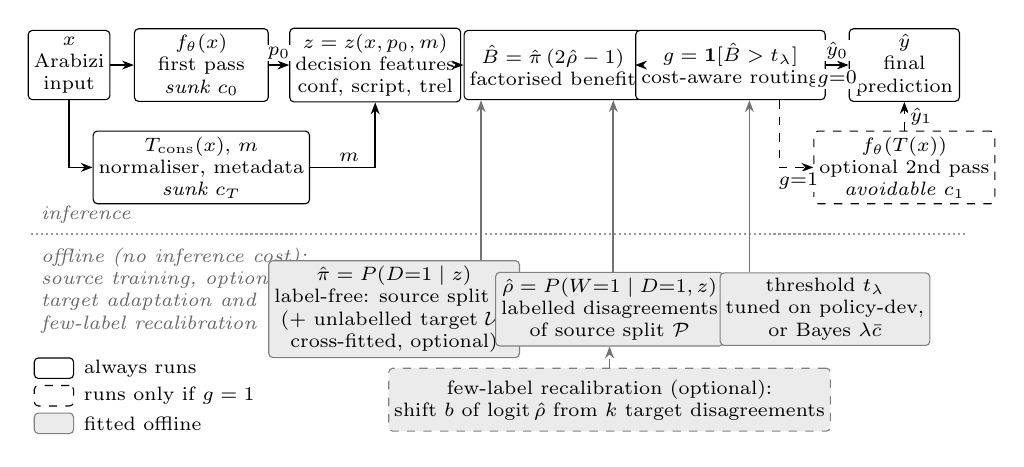
\begin{tikzpicture}[
  x=0.96cm, font=\scriptsize,
  box/.style={draw, rounded corners=1.5pt, align=center, minimum height=8.8mm, inner sep=2pt, fill=white},
  off/.style={box, fill=black!8, draw=black!50, minimum height=8mm},
  arr/.style={-{Stealth[length=1.5mm]}, semithick},
  offarr/.style={arr, black!55},
  lbl/.style={fill=white, inner sep=0.8pt}]
% ---------------- inference lane ----------------
\node[box, minimum width=9mm] (x) at (0,0) {$x$\\Arabizi\\input};
\node[box, minimum width=17mm] (f0) at (1.75,0) {$f_\theta(x)$\\first pass\\\itshape sunk $c_0$};
\node[box, minimum width=17mm] (T) at (1.75,-1.3) {$T_{\rm cons}(x)$, $m$\\normaliser, metadata\\\itshape sunk $c_T$};
\node[box, minimum width=17mm] (z) at (4.05,0) {$z=z(x,p_0,m)$\\decision features\\conf, script, trel};
\node[box, minimum width=19mm] (B) at (6.4,0) {$\hat B=\hat\pi\,(2\hat\rho-1)$\\factorised benefit};
\node[box, minimum width=17mm] (g) at (8.75,0) {$g=\mathbf 1[\hat B>t_\lambda]$\\cost-aware routing};
\node[box, minimum width=14mm] (y) at (11.05,0) {$\hat y$\\final\\prediction};
\node[box, dashed, minimum width=14mm] (f1) at (11.05,-1.3) {$f_\theta(T(x))$\\optional 2nd pass\\\itshape avoidable $c_1$};
\draw[arr] (x) -- (f0);
\draw[arr] (x.south) |- (T.west);
\draw[arr] (f0) -- node[lbl, above=1pt]{$p_0$} (z);
\draw[arr] (T.east) -| node[lbl, pos=.3, above=1pt]{$m$} (z.south);
\draw[arr] (z) -- (B);
\draw[arr] (B) -- (g);
\draw[arr] (g) -- node[lbl, above=1pt]{$\hat y_0$} node[lbl, below=1pt]{$g{=}0$} (y);
\draw[arr, dashed] ($(g.south)+(0.65,0)$) |- node[lbl, pos=.78, below=1pt]{$g{=}1$} (f1.west);
\draw[arr, dashed] (f1) -- node[lbl, right=1pt]{$\hat y_1$} (y);
% ---------------- lane separator ----------------
\draw[black!40, densely dotted, thick] (-0.5,-2.15) -- (11.85,-2.15);
\node[anchor=south west, font=\scriptsize\itshape, text=black!60] at (-0.5,-2.13) {inference};
\node[anchor=north west, font=\scriptsize\itshape, text=black!60, align=left] at (-0.5,-2.2) {offline (no inference cost):\\source training, optional\\target adaptation and\\few-label recalibration};
% ---------------- offline lane ----------------
\node[off] (pi) at (4.3,-3.1) {$\hat\pi=P(D{=}1\mid z)$\\label-free: source split $\mathcal P$\\($+$ unlabelled target $\mathcal U$,\\cross-fitted, optional)};
\node[off] (rho) at (7.15,-3.1) {$\hat\rho=P(W{=}1\mid D{=}1,z)$\\labelled disagreements\\of source split $\mathcal P$};
\node[off] (thr) at (10.0,-3.1) {threshold $t_\lambda$\\tuned on policy-dev,\\or Bayes $\lambda\bar c$};
\node[off, dashed] (fl) at (7.15,-4.25) {few-label recalibration (optional):\\shift $b$ of $\operatorname{logit}\hat\rho$ from $k$ target disagreements};
\draw[offarr] (5.45,0 |- pi.north) -- (5.45,0 |- B.south);
\draw[offarr] (7.2,0 |- rho.north) -- (7.2,0 |- B.south);
\draw[offarr] (9.0,0 |- thr.north) -- (9.0,0 |- g.south);
\draw[offarr, dashed] (fl) -- (rho);
% ---------------- legend ----------------
\node[box, minimum width=5mm, minimum height=2.6mm, inner sep=0pt] (l1) at (-0.2,-3.85) {};
\node[anchor=west] at (l1.east) {always runs};
\node[box, dashed, minimum width=5mm, minimum height=2.6mm, inner sep=0pt] (l2) at (-0.2,-4.2) {};
\node[anchor=west] at (l2.east) {runs only if $g=1$};
\node[off, minimum width=5mm, minimum height=2.6mm, inner sep=0pt] (l3) at (-0.2,-4.55) {};
\node[anchor=west] at (l3.east) {fitted offline};
\end{tikzpicture}

\Description{Block diagram of SelectNorm. Upper lane, inference: the Arabizi input x goes to the first pass of the frozen classifier and to the conservative normaliser with metadata, whose costs c0 and cT are sunk; both feed the decision features z, then the factorised benefit, then cost-aware routing. If g is 0, the first-pass prediction is returned; if g is 1, a dashed optional second pass on T(x), with avoidable cost c1, produces the prediction. Lower lane, offline: the disagreement estimator, the conditional advantage estimator, the threshold and the optional few-label recalibration.}
\caption{SelectNorm. Upper lane (inference): $f_\theta(x)$ and $\Tcons(x)$ always run, so $c_0$ and $c_T$ are incurred before the decision $g$; the dashed second pass $f_\theta(T(x))$ is the only avoidable cost and runs only when $g=1$. Lower lane (grey, offline): $\hat\pi$ (label-free, optionally adapted on unlabelled target text), $\hat\rho$ (source disagreements), the threshold $t_\lambda$ and the optional few-label shift of $\hat\rho$.}
\label{fig:arch}
\end{figure}

\paragraph{Module A: conservative normaliser.}
$T$ changes only Latin-script tokens (Algorithm~\ref{alg:norm}). A token is looked up in a lexicon of Arabizi$\to$CODA pairs built from 80\% of TArC~\cite{gugliotta2022tarc}; unseen tokens fall back to Tunisian character rules (\textit{3}$\to$\ar{ain}, \textit{7}$\to$\ar{hha}, \textit{9}$\to$\ar{qaf}, \textit{5}$\to$\ar{kha}, \textit{ch}$\to$\ar{shin}, word-initial vowels to alef, medial short vowels dropped). Three safeguards define $\Tcons$: (i)~\emph{protection} of French and English tokens, decided from word frequencies against TArC evidence, with short or function-like tokens (\textit{la}, \textit{ma}, \textit{el}) read in the language of their context; (ii)~\emph{negation}: frequent negators (\textit{mouch}, \textit{mech}) are mapped by a fixed list and the circumfix \textit{ma\ldots ch} is split as \ar{ma}\,+\,stem\,+\,\ar{shin}; (iii)~\emph{non-lexical cues}: laughter (\textit{hhhh}, \textit{mdr}) becomes \ar{laugh}. $T_{\rm rule}$ (rules only) and $T_{\rm lex}$ (no safeguards) are controls. Each call also returns token-level metadata $m$ (counts per branch, ambiguous characters).

\paragraph{Module B: benefit estimation.}
The decision-point features $z$ form three groups: \emph{conf} (maximum probability, margin and entropy of the temperature-scaled $p_0$), \emph{script} (length, Latin share, digits used as letters, emoji and upper-case rates) and \emph{trel} (the metadata $m$ as rates per Latin token, and the share of changed tokens). $\hat\pi$ and $\hat\rho$ are logistic regressions on standardised $z$ (gradient boosting as ablation); $\hat\rho$ is fitted on the disagreements of the policy split only (Algorithm~\ref{alg:train}).

\paragraph{Module C: cost-aware routing.}
At inference (Algorithm~\ref{alg:infer}) $\hat B(z)=\hat\pi(z)(2\hat\rho(z)-1)$ is compared with a threshold $t_\lambda$: either the Bayes threshold $\lambda\bar c$ of Eq.~(\ref{eq:bayes}), or, as for every baseline, a threshold tuned for each $\lambda$ on the policy development split. No threshold is tuned on target data. With encoder cost $C_f$, the expected inference cost is $C_f+C_T+O(|z|)+\mathbb E[g]\,C_f$; only the last term is avoidable.

\begin{algorithm}[t]
\small
\caption{Conservative normalisation $\Tcons$}
\label{alg:norm}
\begin{algorithmic}[1]
\Require sentence $x$, lexicon $\mathcal L$, rules $R$, frequency lists $F$
\Ensure $T(x)$, metadata $m$
\State $\tau\gets$ tokens of $x$; $\kappa\gets$ share of foreign tokens in $\tau$ by $F$ vs.\ $\mathcal L$
\For{each Latin-script token $t\in\tau$}
  \If{$t$ is laughter} emit \ar{laugh}
  \ElsIf{$t$ is foreign (if short or function-like: iff $\kappa>\nicefrac12$)} keep $t$
  \ElsIf{$t$ is a listed negator} emit its fixed form
  \ElsIf{$t\in\mathcal L$} emit $\mathcal L(t)$
  \ElsIf{$t$ matches \textit{ma\ldots ch}} emit \ar{ma}\,$R(\text{stem})$\,\ar{shin}
  \Else\ emit $R(t)$ and count ambiguous characters
  \EndIf
  \State update $m$ with the branch taken
\EndFor
\State \Return joined output, $m$
\end{algorithmic}
\end{algorithm}

\begin{figure}[t]
\begin{minipage}[t]{0.555\textwidth}
\begin{algorithm}[H]
\footnotesize
\caption{Training}
\label{alg:train}
\begin{algorithmic}[1]
\Require $f$, $T$, labelled policy split $\mathcal P$; optional: unlabelled target fold $\mathcal U$; $k$ labelled target disagreements $\mathcal K$
\Ensure $\hat\pi$, $\hat\rho$ (and shift $\hat b$)
\For{$x\in\mathcal P\cup\mathcal U$} compute $p_0,p_1$, $z$, $D$ \EndFor
\State $\hat\rho\gets$ fit $P(W{=}1\mid z)$ on $\{i\in\mathcal P: D_i{=}1\}$
\State $\hat\pi\gets$ fit $P(D{=}1\mid z)$ on $\mathcal P$\Statex\hspace{\algorithmicindent}(or on $\mathcal P\cup\mathcal U$, equal total weight)
\If{$\mathcal K\neq\emptyset$} \Comment{few-label shift}
  \State $\hat b\gets\arg\max_b\,\ell(b)$, with $r_i=\operatorname{logit}\hat\rho(z_i)$:\Statex\hspace{\algorithmicindent}\hspace{\algorithmicindent}$\ell(b)=\sum_{\mathcal K}\log\mathrm{Bern}(W_i;\sigma(r_i{+}b))-b^2\!/2$
\EndIf
\end{algorithmic}
\end{algorithm}
\end{minipage}\hfill
\begin{minipage}[t]{0.43\textwidth}
\begin{algorithm}[H]
\footnotesize
\caption{Inference}
\label{alg:infer}
\begin{algorithmic}[1]
\Require $x$, $f$, $T$, $\hat\pi$, $\hat\rho$, threshold $t_\lambda$ ($\lambda\bar c$ or tuned on policy-dev)
\Ensure label $\hat y$, action $g$, score $\hat B$
\State $p_0\gets f(x)$; $(x',m)\gets T(x)$ \Comment{sunk}\State $z\gets z(x,p_0,m)$
\State $\hat B\gets\hat\pi(z)(2\hat\rho(z)-1)$\State $g\gets\mathbf 1[\hat B>t_\lambda]$
\If{$g=1$} $\hat y\gets\mathbf 1[f(x')>\nicefrac12]$
\Else\ $\hat y\gets\mathbf 1[p_0>\nicefrac12]$ \EndIf
\State \Return $\hat y,g,\hat B$
\end{algorithmic}
\end{algorithm}
\end{minipage}
\end{figure}

\section{Experimental Setup}
\label{sec:setup}

\begin{table}[t]
\centering
\caption{Data after de-duplication and near-copy removal (character 3-gram cosine $\ge0.9$ against every training or policy sentence). $S_5^{\textsc{ar}}$: human Arabic-script transliteration of $S_5$~\cite{touileb2021interplay}.}
\label{tab:data}
\footnotesize\setlength{\tabcolsep}{4pt}
\begin{tabular}{@{}llrrl@{}}
\toprule
Set & Variety, script & $N$ & Pos.\% & Role\\
\midrule
TSAC-\textsc{ar} & Tunisian, Arabic & 5{,}564 & 45.0 & train $f$ (90/10)\\
TSAC-\textsc{lat} train & Tunisian, Latin & 6{,}204 & 57.3 & policy pool\\
$S_3$ TSAC-\textsc{lat} test & Tunisian, Latin & 1{,}425 & 55.2 & test\\
$S_4$ TUNIZI & Tunisian, Latin & 2{,}875 & 48.8 & test\\
$S_5$ NArabizi & Algerian, Latin & 729 & 52.0 & test\\
$S_5^{\textsc{ar}}$ NArabizi gold & Algerian, Arabic & 729 & 52.0 & RQ4\\
$S_6$ MYC-\textsc{lat} & Moroccan, Latin & 4{,}191 & 66.4 & test\\
\bottomrule
\end{tabular}
\end{table}

\paragraph{Data and classifiers.}
$f$ is trained on Arabic-script TSAC~\cite{medhaffar2017tsac}; the human Latin-script TSAC training comments, never seen by $f$, form the policy pool (Table~\ref{tab:data}). Test sets cover the same corpus ($S_3$), another Tunisian corpus and platform ($S_4$, TUNIZI~\cite{fourati2021tunizi}), Algerian ($S_5$, NArabizi~\cite{seddah2020narabizi,touileb2021interplay}) and Moroccan Arabizi ($S_6$, MYC~\cite{jbel2023myc}). Mixed-script sentences (minority alphabet $>20\%$) are excluded; corpora were cloned at fixed commits and are not redistributed. $f_\theta$ is a logistic regression on mean-pooled frozen representations of XLM-R base~\cite{conneau2020xlmr}, mE5 base~\cite{wang2024me5}, LaBSE~\cite{feng2022labse} or MARBERTv2~\cite{abdulmageed2021marbert} at pinned revisions, with regularisation and a temperature~\cite{guo2017calibration} fitted on the 10\% Arabic-script development split. No encoder is fine-tuned and no Latin-script sentence trains $f$. In an exploratory regime (\textsc{+syn}), logged as a deviation before it was run, $f$ also sees a synthetic Latin rendering of each training sentence.

\paragraph{Systems.}
B0 keeps $x$; B1 always normalises with $\Tcons$; B2 routes at random at SelectNorm's selection rate (20 draws); B3 thresholds the confidence of $p_0$; B4 estimates $B(z)$ directly as $P(\text{help}\mid z)-P(\text{harm}\mid z)$, a post-hoc deferral rule~\cite{jitkrittum2023cascade}; B4b predicts each view's error~\cite{kim2020learningloss}; B6 is the oracle; R averages both views' probabilities. SelectNorm-src uses source estimates; SelectNorm-adapt, the primary system, re-estimates $\hat\pi$ on unlabelled target text with two-fold cross-fitting by source sentence. All thresholds are tuned per $\lambda$ on the policy development split (the Bayes threshold $\lambda\bar c$ is a variant); nothing is tuned on a test set.

\paragraph{Few-label setting.}
Each test set is split into two folds by source sentence; to predict one fold, $k\in\{8,\ldots,128\}$ labels are drawn from the other, at random or among its disagreements, and re-estimate $b$ (SelectNorm), re-fit B4, re-tune B3, or choose B0 or B1 for the fold (set-level choice). A replay of all 8{,}000 draws, checked against indices logged by a rerun, found no sentence whose own label informed its prediction. On $S_5$ at $k{=}128$ only 97--116 disagreements exist per fold, so 375 targeted draws are smaller than $k$. Each $k$ uses 5 draws $\times$ 5 seeds and the $\lambda=0$ threshold.

\paragraph{Mechanisms, statistics and costs.}
We measure (M1) the AUC of $\hat\pi$ for disagreements; (M2) the AUC of $\hat\rho$ for the winning view among disagreements, its calibration gap, and a ceiling from 5-fold cross-validation of $\hat\rho$ on \emph{target} labels; (M3) the gain over the best view of the rule $\hat\rho>\nicefrac12$; (M4) the oracle headroom, against the headroom between two classifiers trained on bootstrap resamples and applied to the same input. Intervals are 95\% percentile intervals from 1{,}000 seed-averaged bootstrap resamples of test sentences, without refitting. Macro-F1 is primary; results average five seeds, which fix the policy split and random draws. Differences are tested with a paired bootstrap over source sentences~\cite{koehn2004bootstrap,dror2018hitchhiker} (10{,}000 resamples) with Holm correction over the 20 main comparisons per encoder. A difference is \emph{relevant} if it is at least one point and significant after correction; the protocol's wording requires only the unadjusted interval to exclude zero, which coincides in the primary regime (for \textsc{+syn} we report both). Non-significance is not read as equivalence. Costs are relative to one pass of $f$ on $x$: $c_T$ is measured; $c_0,c_1$ are \emph{estimated} by a per-encoder model $a+b\cdot\text{tokens}$ fitted to measured batch-1 CPU latencies and checked by end-to-end timing.

\paragraph{Status of analyses.}
Pre-specified: main comparisons and statistics, the $\lambda$ grid, the embedding, boosting and $T_{\rm lex}$ ablations, the few-label setting and RQ4. Exploratory, logged after the first mE5 results: $T_{\rm cov}$, \textsc{+syn} and M1--M4. Added in revision: mechanism intervals, sensitivity and equivalence readings, end-to-end timing, the normaliser audit and the input-dependent cost threshold.

\section{Results}
\label{sec:results}

\begin{table}[t]
\centering
\caption{Macro-F1 ($\lambda=0$, mean of five seeds), classifier trained on Arabic script only. Bold: best deployable system per column; shaded: SelectNorm-adapt (primary). $^{\triangledown}$/$^{\blacktriangle}$: baseline significantly worse/better than SelectNorm-adapt (paired bootstrap, Holm-corrected $p<0.05$ over 20 comparisons per encoder; tested for B0, B1, B3, B4, SelectNorm-src). $^\dagger$Two passes; $^\ddagger$uses test labels.}
\label{tab:main}
\footnotesize\setlength{\tabcolsep}{3.2pt}
\begin{tabular}{@{}lrrrrrrrr@{}}\toprule
 & \multicolumn{4}{c}{\textbf{mE5}} & \multicolumn{4}{c}{\textbf{XLM-R}}\\
\cmidrule(lr){2-5}\cmidrule(lr){6-9}
 & $S_3$ & $S_4$ & $S_5$ & $S_6$ & $S_3$ & $S_4$ & $S_5$ & $S_6$\\\midrule
B0 original & 63.4$^{\triangledown}$ & 61.5$^{\triangledown}$ & 63.6$^{\triangledown}$ & \textbf{54.1} & 54.5$^{\triangledown}$ & 48.8$^{\triangledown}$ & 48.6$^{\triangledown}$ & 63.5$^{\triangledown}$\\
B1 always normalise & \textbf{82.0} & \textbf{67.2} & 69.4 & 52.9 & 72.8 & \textbf{64.5} & 63.1 & 72.3$^{\blacktriangle}$\\
B2 random, matched rate & 80.0 & 66.5 & 68.5 & 53.2 & 70.2 & 63.3 & 61.9 & 68.9\\
B3 confidence threshold & 82.0 & 67.2 & 69.4 & 52.9 & 72.9 & 64.4 & 63.0 & \textbf{72.3}$^{\blacktriangle}$\\
B4 direct gain & 81.4 & 67.0 & 69.9 & 53.6 & 73.5 & 63.9 & 63.3 & 68.7\\
B4b per-view loss & 81.6 & 67.1 & 69.9 & 53.7 & \textbf{73.9} & 63.9 & \textbf{63.4} & 68.2\\
SelectNorm-src & 81.3 & 67.0 & \textbf{70.0} & 53.7 & 73.8 & 63.8 & 63.4$^{\blacktriangle}$ & 68.0$^{\triangledown}$\\
\rowcolor{black!6}SelectNorm-adapt & 81.3 & 66.9 & 69.8 & 53.7 & 73.8 & 63.8 & 63.1 & 68.5\\
\quad Bayes threshold $\lambda\bar c$ & 81.4 & 66.9 & 69.6 & 53.5 & 73.9 & 64.0 & 63.4 & 69.0\\
\addlinespace[2pt]
R two-view ensemble$^\dagger$ & 78.9 & 66.5 & 69.7 & 54.4 & 67.3 & 57.2 & 54.7 & 69.7\\
B6 oracle$^\ddagger$ & 90.0 & 81.3 & 81.8 & 63.8 & 83.1 & 75.2 & 70.4 & 82.1\\
\midrule[\heavyrulewidth]
 & \multicolumn{4}{c}{\textbf{LaBSE}} & \multicolumn{4}{c}{\textbf{MARBERTv2}}\\
\cmidrule(lr){2-5}\cmidrule(lr){6-9}
 & $S_3$ & $S_4$ & $S_5$ & $S_6$ & $S_3$ & $S_4$ & $S_5$ & $S_6$\\\midrule
B0 original & 69.6$^{\triangledown}$ & 61.1$^{\triangledown}$ & 65.6$^{\triangledown}$ & \textbf{63.4}$^{\blacktriangle}$ & 64.3$^{\triangledown}$ & 62.4$^{\triangledown}$ & 60.0 & 52.5$^{\triangledown}$\\
B1 always normalise & 83.6 & \textbf{69.1} & 70.9 & 55.5$^{\triangledown}$ & 82.1 & 67.7 & 62.3 & 58.3\\
B2 random, matched rate & 81.0 & 67.3 & 69.5 & 60.4 & 79.9 & 67.3 & 61.9 & 56.7\\
B3 confidence threshold & 83.7 & 69.1 & 70.9 & 55.9$^{\triangledown}$ & \textbf{82.3} & 68.1 & 62.3 & \textbf{58.3}\\
B4 direct gain & 83.4 & 68.6 & 71.6 & 60.6 & 82.1 & 68.2 & \textbf{63.0} & 57.6\\
B4b per-view loss & 83.3 & 68.9 & \textbf{71.6} & 60.5 & 82.1 & 68.1 & 62.8 & 57.6\\
SelectNorm-src & 83.4 & 68.7 & 71.1 & 60.4$^{\triangledown}$ & 82.2 & 68.3 & 62.9 & 57.7\\
\rowcolor{black!6}SelectNorm-adapt & 83.4 & 68.8 & 71.5 & 60.9 & 82.1 & \textbf{68.3} & 62.9 & 57.7\\
\quad Bayes threshold $\lambda\bar c$ & \textbf{83.7} & 68.8 & 71.3 & 60.8 & 82.2 & 68.1 & 62.5 & 57.9\\
\addlinespace[2pt]
R two-view ensemble$^\dagger$ & 81.7 & 68.4 & 72.1 & 60.5 & 82.3 & 69.7 & 62.4 & 58.4\\
B6 oracle$^\ddagger$ & 91.5 & 82.2 & 85.7 & 75.2 & 93.6 & 84.2 & 77.6 & 70.4\\
\bottomrule\end{tabular}

\end{table}

\subsection{Selective normalisation against strong baselines (RQ1, RQ2)}
\label{sec:main-results}
Always normalising (B1) improves over the original input on the Tunisian and Algerian sets for every encoder, by 2.3--18.6 points (Table~\ref{tab:main}); on MYC it gains 8.8 points with XLM-R and loses 7.9 with LaBSE. Learned routing adds no consistent improvement. Against the direct-gain router B4 no difference is significant, and every 95\% interval lies inside $[-0.63,+0.58]$, within the 1-point margin in all 16 cells (a post hoc equivalence reading; Table~S1); SelectNorm-adapt and -src differ by $-0.25$ to $+0.54$ (three small differences significant). Against B1 and B3, SelectNorm-adapt is relevantly better in one cell (LaBSE, MYC: $+5.5$, $+5.0$), where normalising harms and thresholding fails to stop it, and relevantly worse in one (XLM-R, MYC: $-3.8$), where the router keeps the original view for about 40\% of inputs although normalising is right; in the LaBSE MYC cell it is also relevantly worse than B0, the better view there ($-2.5$). Elsewhere only 4 (B1) and 6 (B3) of 16 intervals lie within $\pm1$, and the other non-significant ones span $-1.3$ to $+2.4$, so small gains or losses cannot be excluded.

\subsection{Accuracy and cost (RQ3)}
\label{sec:cost}
\begin{figure}[t]
\centering
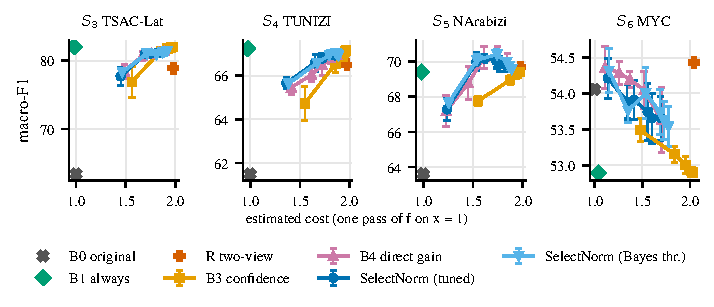
\includegraphics[width=\textwidth]{figures/pareto_lncs.pdf}
\Description{Four panels, one per test set, plotting macro-F1 against estimated inference cost for confidence thresholding, the direct-gain router and SelectNorm with tuned and Bayes thresholds, with single points for B0, B1 and the two-view ensemble.}
\caption{Macro-F1 against estimated cost (mE5, batch size 1, CPU; one pass of $f$ on $x$ = 1) for $\lambda\in\{0,.01,.02,.05,.1,.2\}$; bars: s.d.\ over seeds. Routers and B3 are charged the first pass and the normaliser (sunk) plus the second pass when selected; B1 the normaliser and one pass; R both passes.}
\label{fig:pareto}
\end{figure}
B0 costs 1.00 and B1 0.97--1.04 passes on $x$ (the normaliser adds about 0.4\%). At $\lambda=0$ SelectNorm-adapt costs 1.69--1.88 passes for mE5 and 1.43--1.88 across encoders, against 1.89--2.05 for the ensemble; raising $\lambda$ lowers the cost (mE5: 1.14--1.45 at $\lambda=0.2$) while macro-F1 falls towards B0 (Fig.~\ref{fig:pareto}). Routing is never cheaper than the better single view and never relevantly more accurate (at most $+0.6$, not significant); it saves compute only relative to running both views. End-to-end timing of the deployed pipeline (200 sentences per set; live decisions reproduce all 184{,}400 archived ones) agrees: B0 22--31\,ms; B1 0.91--1.05, SelectNorm-adapt 1.31--1.97, R 1.91--2.07 passes. Thresholding with each input's own cost $\lambda c_1(x)$ (exploratory) changes macro-F1 by $-2.0$ to $+0.6$ and cost by 0 to $-0.11$ passes, moving operating points along the same frontier (no worse on both in 29 of 80 cells, trading accuracy for cost in 48).

\subsection{Where per-input routing fails (RQ5)}
\label{sec:mechanism}
\begin{table}[t]
\centering
\caption{Mechanisms ($\Tcons$, Arabic-script $f$, five seeds). M1: disagreement rate (\%), AUC of target-cross-fitted $\hat\pi$. M2: win rate of $T(x)$ on disagreements (\%), AUC of source and of target-CV $\hat\rho$ (not deployable), calibration gap of source $\hat\rho$. M3: gain over the best view of $\hat\rho>\nicefrac12$. M4: oracle headroom, and the same minus the bootstrap-classifier reference. $^\circ$: AUC interval contains 0.5; $^{*}$: interval excludes 0 (95\%; Table~S4).}
\label{tab:mechanism}
\scriptsize\setlength{\tabcolsep}{2.6pt}
\begin{tabular}{@{}llrrrrrrrrrr@{}}\toprule
 & & \multicolumn{2}{c}{(M1) disagreement} & \multicolumn{4}{c}{(M2) direction} & \multicolumn{2}{c}{(M3) benefit} & \multicolumn{2}{c}{(M4) headroom}\\
\cmidrule(lr){3-4}\cmidrule(lr){5-8}\cmidrule(lr){9-10}\cmidrule(lr){11-12}
Enc. & Set & $P(D)$ & AUC$_\pi$ & $P(W|D)$ & AUC$_\rho$ & AUC$_\rho^{\rm tgt}$ & gap & $\Delta_{\rm src}$ & $\Delta_{\rm tgt}$ & oracle & vs.\ ref.\\\midrule
mE5 & $S_3$ & 34 & 0.68 & 77 & 0.66 & 0.64 & +3 & -0.6$^{*}$ & +0.0 & 8.0 & -0.3\\
 & $S_4$ & 33 & 0.64 & 57 & 0.56 & 0.58 & +19$^{*}$ & -0.3 & -0.1 & 14.1 & +4.6\\
 & $S_5$ & 29 & 0.62 & 58 & 0.63 & 0.57$^\circ$ & +15$^{*}$ & +0.2 & +0.7 & 12.4 & +3.2\\
 & $S_6$ & 21 & 0.74 & 47 & 0.54 & 0.56 & +20$^{*}$ & -0.5 & +0.2 & 9.7 & +4.6\\
\midrule
XLM-R & $S_3$ & 36 & 0.64 & 72 & 0.71 & 0.68 & +3 & +1.0$^{*}$ & +0.8 & 10.3 & +5.9\\
 & $S_4$ & 31 & 0.66 & 64 & 0.57 & 0.57 & +11$^{*}$ & -0.5 & +0.3 & 10.7 & +7.6\\
 & $S_5$ & 23 & 0.69 & 69 & 0.45$^\circ$ & 0.60$^\circ$ & +11$^{*}$ & +0.3 & -0.7 & 7.3 & +2.1\\
 & $S_6$ & 28 & 0.72 & 69 & 0.44 & 0.66 & -8$^{*}$ & -3.3$^{*}$ & +1.1$^{*}$ & 9.8 & +4.5\\
\midrule
LaBSE & $S_3$ & 30 & 0.69 & 73 & 0.61 & 0.53$^\circ$ & -0 & +0.1 & -0.1 & 7.9 & +1.3\\
 & $S_4$ & 34 & 0.65 & 62 & 0.57 & 0.59 & +6$^{*}$ & -0.4 & -0.4 & 13.0 & +5.7\\
 & $S_5$ & 34 & 0.65 & 58 & 0.59 & 0.55$^\circ$ & +3 & +0.4 & +0.2 & 14.9 & +7.5\\
 & $S_6$ & 31 & 0.68 & 33 & 0.57 & 0.64 & +16$^{*}$ & -2.6$^{*}$ & +0.8$^{*}$ & 11.8 & +5.3\\
\midrule
MARBERTv2 & $S_3$ & 39 & 0.69 & 70 & 0.63 & 0.60 & +1 & +0.1 & -0.3 & 11.5 & +0.8\\
 & $S_4$ & 37 & 0.71 & 60 & 0.61 & 0.64 & +13$^{*}$ & +0.4 & +2.8$^{*}$ & 16.5 & +2.0\\
 & $S_5$ & 31 & 0.73 & 57 & 0.63 & 0.54$^\circ$ & +13$^{*}$ & +0.2 & +1.1 & 15.3 & +3.6\\
 & $S_6$ & 30 & 0.71 & 59 & 0.55 & 0.63 & +4$^{*}$ & -0.3 & +1.1$^{*}$ & 12.1 & -0.7\\
\bottomrule\end{tabular}

\end{table}
\paragraph{(M1) Disagreement is moderately predictable.} 21--39\% of inputs change label under normalisation; the label-free estimate ranks them with AUC 0.62--0.74, all intervals within $[0.57,0.77]$ (Table~\ref{tab:mechanism}, Fig.~\ref{fig:diagmap}). Target re-estimation helps most on MYC (mE5: 0.67 to 0.74), but at $\lambda=0$ the rule depends on $\hat\rho$ alone.

\paragraph{(M2) Direction is weakly predictable from $z$, even in domain.} Source $\hat\rho$ reaches AUC 0.54--0.71 in 14 of 16 cells (upper bounds $\le0.76$); for XLM-R the interval includes 0.5 on Algerian text and lies below it on Moroccan text ($[0.41,0.48]$). Fitted on target labels by cross-validation, a reference no deployable system has, $\hat\rho$ reaches 0.53--0.68 (upper bounds $\le0.73$; five intervals include 0.5). With linear estimators the features carry little information about direction in any domain tested; better features or estimators are not excluded. What changes across domains is the \emph{level} of $\rho$: the win rate ranges from 33\% to 77\%, and source $\hat\rho$ is miscalibrated out of domain (gaps up to $+20$ points; intervals exclude zero in 11 of 12 cells).

\paragraph{(M3, M4) Benefit and headroom.} The rule $\hat\rho>\nicefrac12$ gains $-3.3$ to $+1.0$ points over the best view with source estimates (one interval above zero, three below) and $-0.7$ to $+2.8$ with the target-CV ceiling (upper bounds $\le+3.9$): most of the gap to the oracle remains when the router is fitted on the target. The oracle gains 7--17 points over the best view, but two classifiers differing only in a bootstrap resample of their training data show 3--15 points of such headroom on the same input; this reference depends on how the classifiers are made (2--6 with 80\% subsamples, 5--22 with weaker regularisation; Table~S5) and is not a decomposition.

\paragraph{Linguistic conditions.} On Tunisian and Algerian sets, always normalising helps less on inputs with many French or English tokens or low lexicon coverage, for every encoder except XLM-R on TUNIZI (French/English); negation and length show no consistent pattern. On MYC every condition changes sign with the encoder (Table~S6).

\subsection{Few target labels (RQ6), normaliser and classifier regime}
\label{sec:fewlabel}
With $k$ labelled target sentences, re-estimating the shift of $\hat\rho$ changes macro-F1 relative to zero-shot SelectNorm-adapt by $-1.4$ to $+1.5$ points across encoders, regimes, sets and $k$ (mean $-0.01$). Although targeted labels are $1/P(D{=}1)$ times more informative about the shift (Proposition~\ref{prop:efficiency}), targeted and random labels give results within $-0.1$ to $+0.2$ points of each other at every $k$ (averaged, descriptive). In the Arabic-script regime SelectNorm beats a set-level choice between B0 and B1 when $k\le16$ (by 2.6--2.9 points on average); the advantage shrinks to 0.3 points at $k=128$, consistent with M2.

\label{sec:normaliser}
The safeguards matter more than routing: always normalising with $T_{\rm lex}$ or $T_{\rm rule}$ loses 4--11 points on every set for mE5, and routing over them recovers only part of the loss (Table~S7). Keeping out-of-lexicon tokens in Latin script ($T_{\rm cov}$) reduces disagreements by about a third; it is worse than $\Tcons$ on the Tunisian sets and slightly better on $S_5$ and $S_6$. On NArabizi (RQ4), B1 agrees with $f$'s prediction on the human transliteration for 73--77\% of inputs, against 61--67\% for B0 and 73--76\% for SelectNorm-adapt; $f$ reaches 65--77 macro-F1 on the human transliterations. In the \textsc{+syn} regime (Table~S2) the original view improves, the win rate on disagreements moves towards 50\%, and SelectNorm-adapt is relevantly better than the better view once with Holm correction (MARBERTv2, $S_4$, $+1.1$) and twice more under the unadjusted criterion (mE5, $S_3$ $+2.1$, $S_4$ $+1.4$), and relevantly worse in two MYC cells under both (LaBSE $-2.4$, MARBERTv2 $-1.8$); it is never significantly better than B4 (worse once, $-0.4$).

\subsection{Qualitative examples}
\label{sec:qualitative}
% Qualitative examples. Values copied from results/qualitative/examples_mE5.json (archived per-example exports,
% re-checked against results/export/per_example and a rerun of T_cons). Provenance: docs/aciids2027/EXAMPLE_PROVENANCE.md
\begin{table}[t]
\centering
\caption{Test sentences with archived predictions (mE5, $\lambda=0$, SelectNorm-adapt): $x$ above $\Tcons(x)$; gold $y$ (1 = positive); posteriors $p_0$, $p_1$; routing $g$ and prediction $\hat y$ for seeds 0--4. Sources: TSAC test-file line (LGPL-3.0); NArabizi \texttt{sent\_id} (UD release, CC BY-SA 4.0); MYC row of \texttt{DATA\_CLEANED.csv}, text withheld (no licence).}
\label{tab:qualitative}
\footnotesize\setlength{\tabcolsep}{3pt}
\renewcommand{\arraystretch}{1.05}
\begin{tabular}{@{}l p{6.65cm} c c c l@{}}
\toprule
Source, effect & Original $x$ / normalised $\Tcons(x)$ & $y$ & $p_0$ & $p_1$ & seeds 0--4\\
\midrule
TSAC neg.\ 796 & \textit{mech 5arej 3lik el role} & 0 & .565 & .127 & $g$ \texttt{11111}\\
\quad help & \ar[0.8]{exAa} & & & & $\hat y$ \texttt{00000}\\
\addlinespace[1pt]
TSAC pos.\ 86 & \textit{Metrobi mouch kif ijale4 la5er} & 1 & .806 & .004 & $g$ \texttt{11111}\\
\quad harm & \ar[0.8]{exAb} & & & & $\hat y$ \texttt{00000}\\
\addlinespace[1pt]
NArabizi 2 & \textit{salem 3alikoum inchalah le pondium et les midailes d'or} & 1 & .175 & .842 & $g$ \texttt{11111}\\
\quad help & \ar[0.8]{exBa} & & & & $\hat y$ \texttt{11111}\\
\addlinespace[1pt]
NArabizi 4609 & \textit{oui le Maroc aktar jahiziya li had tasfiyat la 3ala lmostawa tandimi} & 1 & .519 & .088 & $g$ \texttt{11111}\\
\quad harm & \ar[0.8]{exBb} & & & & $\hat y$ \texttt{00000}\\
\addlinespace[1pt]
MYC 9079 & [withheld] two \textit{ma\ldots ch} negations split as \ar[0.8]{ma}\,\ldots\,\ar[0.8]{shin}, & 1 & .645 & .250 & $g$ \texttt{00111}\\
\quad harm (s2--4) & letter elongations squeezed, emoji kept & & & & $\hat y$ \texttt{11000}\\
\addlinespace[1pt]
MYC 14543 & [withheld] two Latin-script loanwords protected, & 1 & .480 & .302 & $g$ \texttt{00001}\\
\quad both wrong & negated verb split, emoji kept & & & & $\hat y$ \texttt{00000}\\
\bottomrule
\end{tabular}
\end{table}

Table~\ref{tab:qualitative} shows six hand-picked (not representative) test sentences. In TSAC~neg.~796 the negator \textit{mech} is mapped by the fixed list and French \textit{role} is protected; in TSAC~pos.~86, \textit{ijale4} and \textit{la5er} fall back to character rules. In both NArabizi sentences the French article \textit{le} is read as Arabizi (the context is mostly Arabizi) and mapped by the negator list to \ar{la} (\textit{no}), yet the normalised view is right in sentence~2 and wrong in 4609. The router selects the normalised view for all four in every seed: its features do not separate these cases. In MYC~9079 the decision varies with the policy split.

\section{Discussion}
\label{sec:discussion}

\paragraph{Findings.}
Transfer matters in specific cells: for XLM-R on Algerian and Moroccan text, source $\hat\rho$ ranks direction at or below chance, and fitting it on the target turns a loss of up to 3.3 points into a small gain. Elsewhere the limit is in-domain, and richer variants did not change this (16 embedding components: $-1.2$ to $+1.1$, no consistent sign; gradient boosting, mE5 only: $-0.6$ to $+0.7$). The win rate on disagreements varies far more between encoder--dialect pairs (33--77\%) than our features resolve within a set, and with 64--128 target labels a set-level choice is on average within 0.3--0.7 points of SelectNorm with the same labels (descriptive). The factorisation adds a diagnosis, not an accuracy gain.

\paragraph{Explanations.}
Our reading is that decision-point features say little about which view is right, and that much of the oracle headroom is of the size classifier variability alone produces (M4). These are limits of the features and estimators evaluated; other features, fine-tuned representations or estimators might do better, and the results do not show that the conditional advantage is intrinsically unpredictable. Targeted labels estimate the shift more efficiently but cannot repair a weak ranking. Transliteration is known to help unseen scripts on average~\cite{muller2021unseen,moosa2023transliteration}; on Moroccan text its sign changes with the encoder. In practice, safeguards matter more than routing, and normalising is best decided per corpus or dialect.

\section{Limitations}
\label{sec:limitations}
\emph{Task and models.} All experiments use binary sentiment, where the factorisation is exact with $\rho$ alone; the $K$-class form needs two conditional win rates. Encoders are frozen and heads linear, and all conclusions are restricted to this setting; fine-tuning could change how often normalisation helps and how predictable the winning view is. We did not fine-tune (CPU only); \textsc{+syn} is only a partial probe.
\emph{Normaliser.} $T$ is built from Tunisian resources (TArC lexicon, Tunisian digit conventions such as \textit{8}\,=\,\ar{ha}). Its safeguards were tuned on the TArC held-out split and no independent transliteration test set was available, so its intrinsic accuracy is \emph{not independently validated}; it is lower on Algerian NArabizi, and with no Moroccan transliteration gold its validity on MYC is unmeasured.
\emph{Data.} Cross-corpus differences mix dialect with platform, topic, period and label distribution; we do not attribute them to dialect alone. TUNIZI, the NArabizi sentiment layer and MYC state no licence, and MARBERTv2 has none on its model card; we use them for research only and do not redistribute them.
\emph{Development.} The pipeline was first exercised with a character $n$-gram classifier whose test results we inspected; this motivated the few-label setting.
\emph{Analysis.} Mechanism intervals cover test-sentence resampling, not estimator refitting; the target-label ceiling uses linear $\hat\rho$ on the same features. Features computed after $f(T(x))$ were not studied, as they need the second pass on every input. Equivalence statements are post hoc and not corrected for multiplicity. The qualitative examples are hand-picked.
\emph{Costs.} Costs are estimated from a token-length model and checked by timing 200 sentences per set on one 4-core CPU; relative costs on accelerators differ, especially for short inputs.

\section{Conclusion}
\label{sec:conclusion}
We studied per-input normalisation of Arabizi for frozen encoders with linear heads, using the disagreement factorisation of the expected benefit as an analysis device. Normalisation improves macro-F1 on Tunisian and Algerian Arabizi, and its effect on Moroccan text depends on the encoder. Learned per-input routing, including SelectNorm, does not consistently exceed the better single view or strong baselines, and it costs more than either single view because the first pass is sunk. Measured separately, disagreement is moderately predictable from decision-point features, whereas the conditional advantage of the normalised view is weakly predictable under the features and estimators evaluated, also when fitted on target labels. The usable signal is mostly set-level, which about a hundred target labels recover.

\paragraph{Code and Reproducibility.}
Code, configuration, the pre-registered protocol, logs, per-example predictions, supplementary Tables~S1--S8 and all figure data are at \url{[GITHUB_REPOSITORY_URL]}, with dependencies, commands, pinned encoder revisions and corpus commits, and instructions for obtaining the corpora, which are not redistributed. A script recomputes every test of Table~\ref{tab:main} from the exports. Quoted NArabizi sentences are from the UD release \url{https://github.com/UniversalDependencies/UD_Maghrebi_Arabic_French-Arabizi} (CC BY-SA 4.0); quoted TSAC sentences are from \url{https://github.com/fbougares/TSAC} (LGPL-3.0).

\begin{credits}
\subsubsection{\discintname}
[To be confirmed by the authors.] The authors have no competing interests to declare that are relevant to the content of this article.
\end{credits}

%
\bibliographystyle{splncs04}
\bibliography{references}
%
\appendix
\section{Proofs}
\label{app:proofs}

\paragraph{Bayes rule and factorisation.}
For fixed $z$, the conditional risk of $g(z)=a$ is $\mathbb E[e_a\mid z]+\lambda\,\mathbb E[c_0+c_T\mid z]+\lambda\bar c(z)\,a$; the middle term does not depend on $a$, so $a=1$ is strictly better iff $B(z)>\lambda\bar c(z)$, and pointwise minimisation minimises Eq.~(\ref{eq:risk}). If $D=0$, $e_0=e_1$; if $D=1$ and $y\in\{0,1\}$, $e_0=W$ and $e_1=1-W$. Hence $e_0-e_1=D(2W-1)$ and $B(z)=P(D{=}1\mid z)\big(2P(W{=}1\mid D{=}1,z)-1\big)$; for $K$ classes $e_0-e_1=D\big(\mathbf 1[\hat y_1{=}y]-\mathbf 1[\hat y_0{=}y]\big)$ gives $\pi(\rho_1-\rho_0)$. \qed

\paragraph{Proposition~\ref{prop:regret}.}
Where $\hat g(z)\neq g^\star(z)$, the conditional excess risk is $|B-\lambda\bar c|\le|\hat B-B|$, because $\hat B-\lambda\bar c$ and $B-\lambda\bar c$ differ in sign (or $\hat B=\lambda\bar c$). Hence $R(\hat g)-R(g^\star)\le\mathbb E|\hat B-B|$, and $\hat B-B=(\hat\pi-\pi)(2\rho-1)+2\hat\pi(\hat\rho-\rho)$ with the triangle inequality concludes. \qed

\paragraph{Proposition~\ref{prop:efficiency}.}
With $q_i=\sigma(\operatorname{logit}\hat\rho(z_i)+b)$, a labelled target example contributes the log-likelihood $D_i[W_i\log q_i+(1-W_i)\log(1-q_i)]$ (if $D_i=0$, $e_0=e_1$ whatever $y_i$), hence Fisher information $D_i\,q_i(1-q_i)$ about $b$. Its expectation is $P_Q(D{=}1)\,\mathbb E_Q[q(1-q)\mid D{=}1]$ under random sampling and $\mathbb E_Q[q(1-q)\mid D{=}1]$ among disagreements (sampled without labels, as $D$ is observable); information adds over draws. \qed

\section{Disagreement--Advantage Diagnostic Map}
\label{app:diagmap}
\begin{figure}[H]
\begin{minipage}[c]{0.47\textwidth}
% generated by diagnostic_map.py from diagnostic_map.csv; do not edit by hand
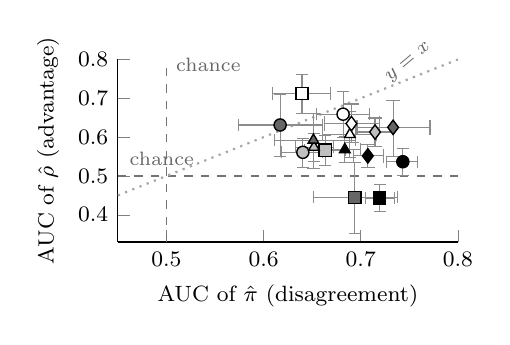
\begin{tikzpicture}
\begin{axis}[width=5.9cm, height=3.9cm, xmin=0.45, xmax=0.80, ymin=0.33, ymax=0.80,
  xlabel={AUC of $\hat\pi$ (disagreement)}, ylabel={AUC of $\hat\rho$ (advantage)},
  label style={font=\footnotesize}, tick label style={font=\footnotesize}, xtick={0.5,0.6,0.7,0.8}, ytick={0.4,0.5,0.6,0.7,0.8},
  axis lines*=left, clip=false, legend cell align=left, 
  error bars/error bar style={black!45, line width=0.4pt}]
\draw[black!55, dashed] (axis cs:0.5,0.33) -- (axis cs:0.5,0.80);
\draw[black!55, dashed] (axis cs:0.45,0.5) -- (axis cs:0.80,0.5);
\draw[black!35, dotted, thick] (axis cs:0.45,0.45) -- (axis cs:0.80,0.80);
\node[font=\scriptsize, text=black!60, anchor=south west] at (axis cs:0.50,0.745) {chance};
\node[font=\scriptsize, text=black!60, anchor=south west] at (axis cs:0.452,0.503) {chance};
\node[font=\scriptsize, text=black!60, rotate=40, anchor=south] at (axis cs:0.76,0.76) {$y=x$};
\addplot[only marks, mark=*, mark size=2.2pt, mark options={draw=black, fill=white, line width=0.5pt}, forget plot, error bars/.cd, x dir=both, x explicit, y dir=both, y explicit] coordinates {(0.6818,0.6591) -= (0.0278,0.0598) += (0.0270,0.0572)};
\addplot[only marks, mark=*, mark size=2.2pt, mark options={draw=black, fill=black!25, line width=0.5pt}, forget plot, error bars/.cd, x dir=both, x explicit, y dir=both, y explicit] coordinates {(0.6404,0.5609) -= (0.0216,0.0385) += (0.0202,0.0349)};
\addplot[only marks, mark=*, mark size=2.2pt, mark options={draw=black, fill=black!60, line width=0.5pt}, forget plot, error bars/.cd, x dir=both, x explicit, y dir=both, y explicit] coordinates {(0.6170,0.6312) -= (0.0426,0.0805) += (0.0432,0.0774)};
\addplot[only marks, mark=*, mark size=2.2pt, mark options={draw=black, fill=black, line width=0.5pt}, forget plot, error bars/.cd, x dir=both, x explicit, y dir=both, y explicit] coordinates {(0.7433,0.5366) -= (0.0169,0.0346) += (0.0153,0.0343)};
\addplot[only marks, mark=square*, mark size=2.2pt, mark options={draw=black, fill=white, line width=0.5pt}, forget plot, error bars/.cd, x dir=both, x explicit, y dir=both, y explicit] coordinates {(0.6395,0.7122) -= (0.0299,0.0506) += (0.0290,0.0493)};
\addplot[only marks, mark=square*, mark size=2.2pt, mark options={draw=black, fill=black!25, line width=0.5pt}, forget plot, error bars/.cd, x dir=both, x explicit, y dir=both, y explicit] coordinates {(0.6634,0.5664) -= (0.0213,0.0392) += (0.0205,0.0385)};
\addplot[only marks, mark=square*, mark size=2.2pt, mark options={draw=black, fill=black!60, line width=0.5pt}, forget plot, error bars/.cd, x dir=both, x explicit, y dir=both, y explicit] coordinates {(0.6938,0.4450) -= (0.0426,0.0935) += (0.0437,0.0898)};
\addplot[only marks, mark=square*, mark size=2.2pt, mark options={draw=black, fill=black, line width=0.5pt}, forget plot, error bars/.cd, x dir=both, x explicit, y dir=both, y explicit] coordinates {(0.7195,0.4431) -= (0.0144,0.0347) += (0.0155,0.0338)};
\addplot[only marks, mark=triangle*, mark size=2.2pt, mark options={draw=black, fill=white, line width=0.5pt}, forget plot, error bars/.cd, x dir=both, x explicit, y dir=both, y explicit] coordinates {(0.6888,0.6068) -= (0.0284,0.0598) += (0.0274,0.0587)};
\addplot[only marks, mark=triangle*, mark size=2.2pt, mark options={draw=black, fill=black!25, line width=0.5pt}, forget plot, error bars/.cd, x dir=both, x explicit, y dir=both, y explicit] coordinates {(0.6518,0.5741) -= (0.0192,0.0361) += (0.0198,0.0362)};
\addplot[only marks, mark=triangle*, mark size=2.2pt, mark options={draw=black, fill=black!60, line width=0.5pt}, forget plot, error bars/.cd, x dir=both, x explicit, y dir=both, y explicit] coordinates {(0.6513,0.5923) -= (0.0403,0.0732) += (0.0433,0.0675)};
\addplot[only marks, mark=triangle*, mark size=2.2pt, mark options={draw=black, fill=black, line width=0.5pt}, forget plot, error bars/.cd, x dir=both, x explicit, y dir=both, y explicit] coordinates {(0.6836,0.5679) -= (0.0162,0.0323) += (0.0158,0.0333)};
\addplot[only marks, mark=diamond*, mark size=2.6pt, mark options={draw=black, fill=white, line width=0.5pt}, forget plot, error bars/.cd, x dir=both, x explicit, y dir=both, y explicit] coordinates {(0.6904,0.6348) -= (0.0278,0.0476) += (0.0285,0.0504)};
\addplot[only marks, mark=diamond*, mark size=2.6pt, mark options={draw=black, fill=black!25, line width=0.5pt}, forget plot, error bars/.cd, x dir=both, x explicit, y dir=both, y explicit] coordinates {(0.7147,0.6131) -= (0.0200,0.0373) += (0.0188,0.0362)};
\addplot[only marks, mark=diamond*, mark size=2.6pt, mark options={draw=black, fill=black!60, line width=0.5pt}, forget plot, error bars/.cd, x dir=both, x explicit, y dir=both, y explicit] coordinates {(0.7333,0.6251) -= (0.0372,0.0760) += (0.0380,0.0696)};
\addplot[only marks, mark=diamond*, mark size=2.6pt, mark options={draw=black, fill=black, line width=0.5pt}, forget plot, error bars/.cd, x dir=both, x explicit, y dir=both, y explicit] coordinates {(0.7073,0.5517) -= (0.0151,0.0293) += (0.0165,0.0286)};
\addlegendimage{only marks, mark=*, mark size=2.2pt, mark options={draw=black, fill=white}}\label{dm:mE5}
\addlegendimage{only marks, mark=square*, mark size=2.2pt, mark options={draw=black, fill=white}}\label{dm:XLMR}
\addlegendimage{only marks, mark=triangle*, mark size=2.2pt, mark options={draw=black, fill=white}}\label{dm:LaBSE}
\addlegendimage{only marks, mark=diamond*, mark size=2.2pt, mark options={draw=black, fill=white}}\label{dm:MARBERTv2}
\addlegendimage{only marks, mark=square*, mark size=2.2pt, mark options={draw=black, fill=white}}\label{dm:S3}
\addlegendimage{only marks, mark=square*, mark size=2.2pt, mark options={draw=black, fill=black!25}}\label{dm:S4}
\addlegendimage{only marks, mark=square*, mark size=2.2pt, mark options={draw=black, fill=black!60}}\label{dm:S5}
\addlegendimage{only marks, mark=square*, mark size=2.2pt, mark options={draw=black, fill=black}}\label{dm:S6}
\end{axis}
\end{tikzpicture}

\end{minipage}\hfill
\begin{minipage}[c]{0.5\textwidth}
\Description{Scatter plot with one point per encoder and test corpus. The x-axis is the AUC of the disagreement estimator, between 0.62 and 0.74 for all points; the y-axis is the AUC of the conditional advantage estimator, mostly between 0.54 and 0.71, with two XLM-R points near 0.44. Dashed lines mark chance at 0.5 on both axes, and a dotted diagonal marks equal AUC. Fourteen of sixteen points lie below the diagonal.}
\caption{Disagreement--advantage diagnostic map (data of Table~\ref{tab:mechanism}; bars: 95\% intervals). Marker: \ref{dm:mE5}\,mE5, \ref{dm:XLMR}\,XLM-R, \ref{dm:LaBSE}\,LaBSE, \ref{dm:MARBERTv2}\,MARBERTv2; fill: \ref{dm:S3}\,$S_3$, \ref{dm:S4}\,$S_4$, \ref{dm:S5}\,$S_5$, \ref{dm:S6}\,$S_6$. $x$: AUC of target-cross-fitted $\hat\pi$ (M1); $y$: AUC of source $\hat\rho$ (M2); dashed: chance; dotted: equal AUC. 14 of 16 points lie below the diagonal; the two near 0.44 are XLM-R on $S_5$ and $S_6$. Linear estimators on $z$ only.}
\label{fig:diagmap}
\end{minipage}
\end{figure}

\end{document}
